\begin{frame}[c,parent={cmap:jabuti-software-testing},hasnext=true,hasprev=false]
\label{cmap:metrics-tool}
\label{cmap:measurement-tool}
\label{cmap:software-measurement-tool}
\label{cmap:jabuti-measurement-tool}
\frametitle{Measurement tool}

\insertcmap{Courses-SoftwareTesting-JaBUTi-JaBUTiToolsSoftwareMeasurement}
\end{frame}



\begin{frame}[parent={cmap:jabuti-measurement-tool},hasnext=true,hasprev=true]
\frametitle{Measurement tool}
\label{concept:measurement-tool}
\label{concept:metric-tool}
\label{concept:software-measurement-tool}
\label{concept:jabuti-measurement-tool}

\begin{block:concept}{Software measurement}
\begin{itemize}
	\item<1-> Measurements can be used to define a test strategy:
	\begin{itemize}
		\item Which classes, methods and test requirements should be tested
		first?
	\end{itemize}
\end{itemize}
\end{block:concept}

\begin{block:concept}{Measurement tool}
\begin{itemize}
	\item<2-> JaBUTi implements several metrics to aid the tester in the
	definition of the test strategy:
	\begin{itemize}
		\item Test requirement weight based on dominator and super-block
		analysis.

		\item Static metrics for classes and methods.
	\end{itemize}
\end{itemize}
\end{block:concept}
\end{frame}


\begin{frame}
\frametitle{Measurement tool}

\begin{block}{Example}
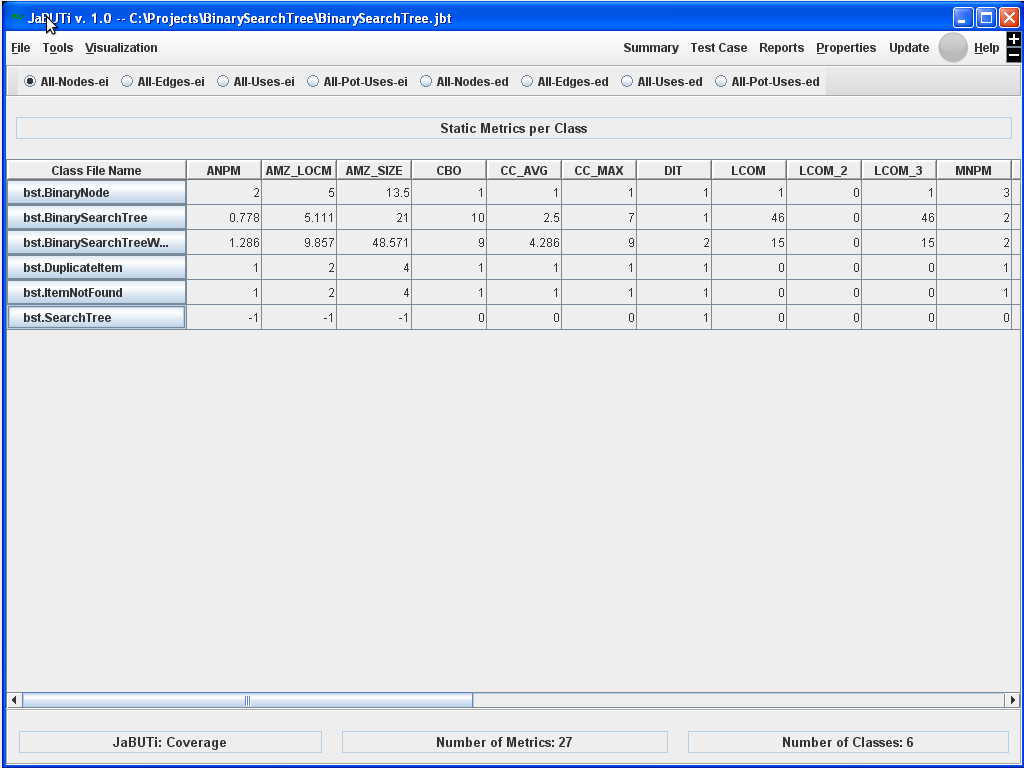
\includegraphics[width=\textwidth,clip]{resources/JaBUTi/JaBUTi-BinarySearchTree/JaBUTi-BinarySearchTree-Metrics}
\end{block}
\end{frame}
